%%%%%%%%%%%%%%%%%%%%%%%%%%%%%%%%%%%%%%%%%
%%% HYPERRIDE Reporting Template
%%%%%%%%%%%%%%%%%%%%%%%%%%%%%%%%%%%%%%%%%

\documentclass[letterpaper,12pt]{report}
\usepackage[pass]{geometry}
\usepackage{hyperride}		% HYPERRIDE specific definitions and styles  
\usepackage[utf8]{inputenc}	% UTF8 package
\usepackage[T1]{fontenc}
\usepackage{textcomp}		% common special chars
\usepackage{amsmath}		% math formula
\usepackage{fancybox}
\usepackage{anyfontsize}	% fonts
\usepackage{lipsum}
\usepackage{float}
\usepackage[normalem]{ulem}
\usepackage{cleveref}
\usepackage[printonlyused]{acronym}
\hypersetup{
	pdftitle={Beacon Network Security Labs: Off-Path TCP Exploits Lab Setup},
	pdfauthor={[Jordan Whyte, Gaby Dagher, Dylan Gresham]},
	pdfkeywords={TCP Exploit, Beacon Labs, Network Security, Off-Path Attacks},
}

\usepackage{subfigure}
\usepackage{graphicx}
\usepackage{xcolor}
\usepackage{soul}
\sethlcolor{lightgray}
\usepackage[export]{adjustbox}
\usepackage{mdframed}
\usepackage{pdfpages}
\usepackage{comment}
\usepackage{multirow,array}
\def\todo#1{{\color{hyperridered}\textbf{TODO:} ``#1''}}
\def\hyperride{HYPERRIDE}
\usepackage{mdframed}
\definecolor{lightblue}{rgb}{0.93, 0.95, 1.0}

\graphicspath{ {graphics/} }

%%%%%%%%%%%%%%%%%%%%%%%%%%%%%%%%%%%%%%%%%
%%% Definitions
%%%%%%%%%%%%%%%%%%%%%%%%%%%%%%%%%%%%%%%%%

\begin{document}


\includepdf[pages=1]{./graphics/Beacon_NS_Module_Page.pdf}

\mdfdefinestyle{code}{%
    linecolor=black,
    outerlinewidth=2pt,
    %roundcorner=20pt,
    innertopmargin=4pt,
    innerbottommargin=4pt,
    innerrightmargin=4pt,
    innerleftmargin=4pt,
        leftmargin = 4pt,
        rightmargin = 4pt
    backgroundcolor=black!10
    }%

\setcounter{tocdepth}{5}
\setcounter{secnumdepth}{5}

%%%%%%%%%%%%%%%%%%%%%%%%%%%%%%%%%%%%%%%%%
%%% URL style same as regular text
%%%%%%%%%%%%%%%%%%%%%%%%%%%%%%%%%%%%%%%%%
	
\urlstyle{same}

%%%%%%%%%%%%%%%%%%%%%%%%%%%%%%%%%%%%%%%%%
%%% Deliverable Information
%%%%%%%%%%%%%%%%%%%%%%%%%%%%%%%%%%%%%%%%%

% Project Meta Information
\ProjectFullTitle{Beacon Network Security Labs: Off-Path TCP Exploits Lab Setup}
\ProjectAcronym{HYPERRIDE}
\ProjectRefNo{957788}

% Report Number, use either "1", "2", or "3" for the corresponding reporting period
\delivNumber{0}

% Period covered by the report
\delivFrom{dd/mm/yyyy}
\delivTo{dd/mm/yyyy}

% Report Responsible Partner
\delivResponsible{AIT Austrian Institute of Technology (AIT)} 

% Report Version, Contractual and Actual Date, Dissemination Level, Type
\delivVersion{vn.n}
\ContractualDate{dd/mm/yyyy}
\ActualDate{dd/mm/yyyy}

% List of Main Authors (usually from the responsible partner)
\delivAuthor{[Jordan Whyte, Gaby Dagher, Dylan Gresham]}

% List of Co-Authors (all other co-authors should be listed here)
\delivFPAuthor{[]}

% Report Status
\delivStatus{d} %% d = draft, f = final, s = submitted

%%%%%%%%%%%%%%%%%%%%%%%%%%%%%%%%%%%%%%%%%
%%% Change Log
%%%%%%%%%%%%%%%%%%%%%%%%%%%%%%%%%%%%%%%%%

\istChange{dd/mm/yyyy}{v1.0}{Name (Partner short name)}{Draft report template}
\istChange{}{}{}{}

%%%%%%%%%%%%%%%%%%%%%%%%%%%%%%%%%%%%%%%%%
%%% Cover Page
%%%%%%%%%%%%%%%%%%%%%%%%%%%%%%%%%%%%%%%%%

%\makecover

%%%%%%%%%%%%%%%%%%%%%%%%%%%%%%%%%%%%%%%%%
%%% Table of Contents
%%%%%%%%%%%%%%%%%%%%%%%%%%%%%%%%%%%%%%%%%

\clearpage
\fancypagestyle{plain}{}
\settableofcontents
\tableofcontents
\clearpage

%%%%%%%%%%%%%%%%%%%%%%%%%%%%%%%%%%%%%%%%%
%%% Overview
%%%%%%%%%%%%%%%%%%%%%%%%%%%%%%%%%%%%%%%%%
\newpage
\section*{Overview}\label{sec:work-carried-out}
\addcontentsline{toc}{section}{Overview}

Guide for setting up the Virtual Machines for the Off-Path TCP and Evil Twin labs.

%%%%%%%%%%%%%%%%%%%%%%%%%%%%%%%%%%%%%%%%%
%%% Virtual Machine Setup
%%%%%%%%%%%%%%%%%%%%%%%%%%%%%%%%%%%%%%%%%

\section*{Virtual Machine Setup}\label{sec:Virtual-Machine-Setup}
\addcontentsline{toc}{section}{Virtual Machine Setup}

For all virtual machines (VMs), it is recommended to allocate at least 15 GB of storage and 2 GB of memory.

\subsection*{Virtual Machine Software Installation}\label{sec:Virtual-Machine-Software-Installation}
\addcontentsline{toc}{subsection}{Virtual Machine Software Installation}

VirtualBox will be the virtual machine software that is used to open the VM images and complete the lab. It is possible to complete the lab with other virtual machine software but it has been untested and so support for other virtual machine software will not be included in this lab document at this point in time.

Begin by downloading Oracle's VirtualBox software. The download links for VirtualBox can be found at the below website.

\url{https://download.virtualbox.org/virtualbox/7.0.18/VirtualBox-7.0.18-162988-Win.exe}

\subsubsection*{Windows Setup}\label{sec:Virtual-Machine-Windows-Setup}
\addcontentsline{toc}{subsubsection}{Windows Setup}

Select the hyperlink titled "Windows hosts" under the "VirtualBox x.x.xx platform packages" to begin the installation of the latest version of VirtualBox. This lab was created when VirtualBox 7.0.18 was the latest release, however, the steps provided should still apply to future versions of VirtualBox as well, the images shown may not be identical, however.

Once the download has completed, run the downloaded installer. The file name should be "VirtualBox-<version\_number>-Win.exe".

Run through the installer without changing anything. At the end, make sure the checkbox is selected to "Start Oracle VM VirtualBox x.x.xx after installation" then click the "Finish" button to complete the installation and open VirtualBox.

\subsubsection*{Linux Setup}\label{sec:Virtual-Machine-Linux-Setup}
\addcontentsline{toc}{subsubsection}{Linux Setup}

Select the hyperlink titled "Linux distributions" under the "VirtualBox <version\_number> platform packages" to navigate to the page containing Oracle's instructions for distribution specific instructions for downloading and installing VirtualBox.

Find your distribution and follow the instructions Oracle has provided.

If your distribution isn't shown on the website, please look into distribution specific instructions for your Linux distro. For example, if you are using Arch Linux, there is a VirtualBox page on the ArchWiki that provides an installation guide.

\subsection*{Off-Path TCP Lab Virtual Machines}\label{sec:Off-Path-TCP-Lab-Virtual-Machines}
\addcontentsline{toc}{subsection}{Off-Path TCP Lab Virtual Machines}

\subsubsection*{Setting up the Virtual Machine Instances}\label{sec:Setting-up-the-Virtual-Machine-Instances}
\addcontentsline{toc}{subsubsection}{Setting up the Virtual Machine Instances}

\paragraph*{Client Virtual Machine Setup}\label{sec:Virtual-Machine-Client-Virtual-Machine-Setup}
\addcontentsline{toc}{paragraph}{Client Virtual Machine Setup}

From the VirtualBox Manager, click the "Import" button, found either on the home page under the Tools banner or in the menu bar under File > Import Appliance. This should open a new window that looks like Figure~\ref{fig:Import_Virtual_Appliance} on page~\pageref{fig:Import_Virtual_Appliance}.

Click the yellow folder icon with a green arrow pointing upwards on the middle-right side of the window to open your operating system's file picker. In this file picker, navigate to where you downloaded the virtual machine .ova images and select "Attacker-002.ova" and then select "Open." The "Attacker-002.ova" image file will be used for both the client and attacker virtual machines.

\begin{figure}[!h]
    \centering
    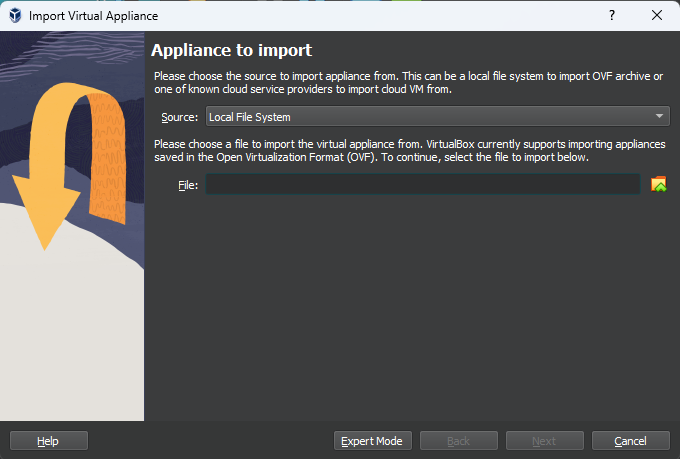
\includegraphics[width=0.9\columnwidth]{graphics/off-path_graphics/import_virtual_appliance.png}
    \caption{Import Virtual Appliance Window}
    \label{fig:Import_Virtual_Appliance}
\end{figure}

To continue on, click the "Next" and then the "Finish" buttons. This will then start the importing appliance job in VirtualBox. Once the job finishes, you'll see a new virtual machine instance in the left titled "Attacker." The VirtualBox Manager should now look similar to Figure~\ref{fig:VirtualBox_Manager_Client_Unnamed} shown on page~\pageref{fig:VirtualBox_Manager_Client_Unnamed}.

\begin{figure}[!h]
    \centering
    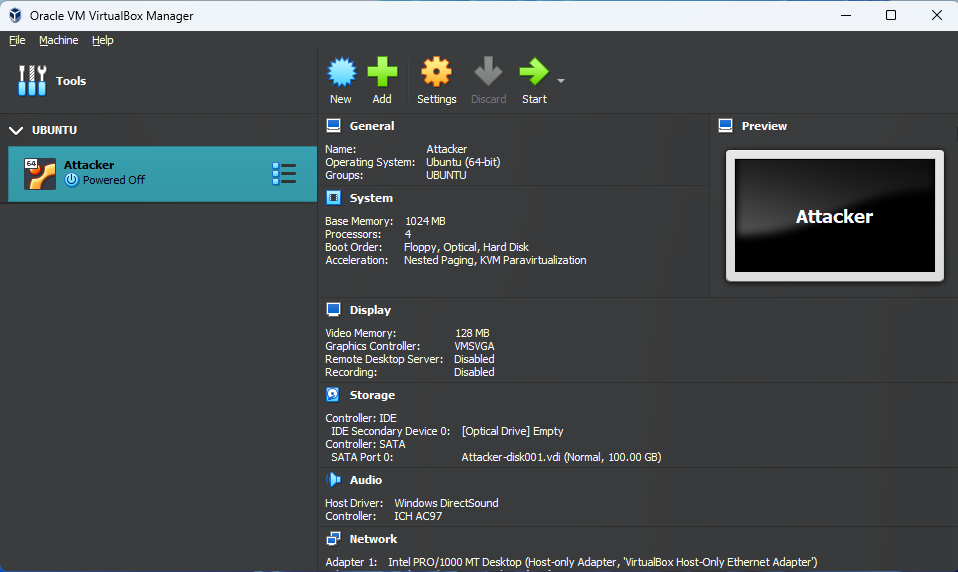
\includegraphics[width=0.9\columnwidth]{graphics/off-path_graphics/virtualbox_manager_client_unnamed.png}
    \caption{VirtualBox Manager with Client VM freshly imported}
    \label{fig:VirtualBox_Manager_Client_Unnamed}
\end{figure}

Select the imported virtual machine instance and click the "Settings" cog in the top-middle of the window. In the window that pops up, under General > Basic > Name, enter "Client VM" and then select the "OK" button. The VirtualBox Manager should now look like Figure~\ref{fig:VirtualBox_Manager_Client_Named} below.

\begin{figure}[!h]
    \centering
    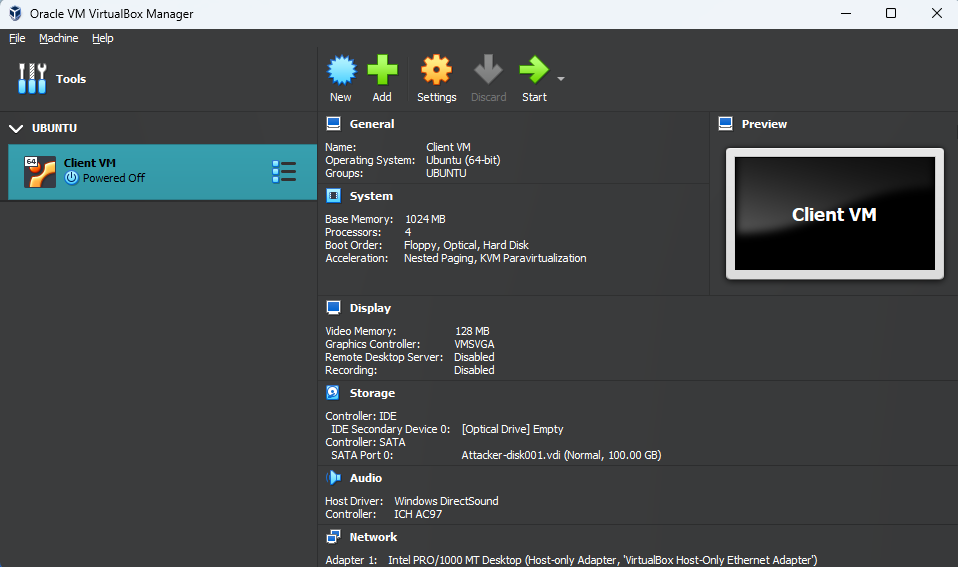
\includegraphics[width=0.9\columnwidth]{graphics/off-path_graphics/virtualbox_manager_client_named.png}
    \caption{VirtualBox Manager with Client VM properly named}
    \label{fig:VirtualBox_Manager_Client_Named}
\end{figure}

\paragraph*{Attacker Virtual Machine Setup}\label{sec:Virtual-Machine-Attacker-Virtual-Machine-Setup}
\addcontentsline{toc}{paragraph}{Attacker Virtual Machine Setup}

From the VirtualBox Manager, click the File option in the menu bar at the top then select the import appliance option from the drop down. Optionally, press Ctrl + I instead to open the Import Virtual Appliance window instead.

Click the yellow folder icon with a green arrow pointing upwards on the middle-right side of the window to open your operating system's file picker. In this file picker, navigate to where you downloaded the virtual machine .ova images to and select "Attacker-002.ova" and then select "Open."

To continue on, click the "Next" and then the "Finish" buttons. This will then start the importing appliance job in VirtualBox. Once the job finishes, you'll see a new virtual machine instance in the left titled "Attacker." The VirtualBox Manager should now look similar to Figure~\ref{fig:VirtualBox_Manager_Client_Attacker} shown on page~\pageref{fig:VirtualBox_Manager_Client_Attacker}.

\begin{figure}[!h]
    \centering
    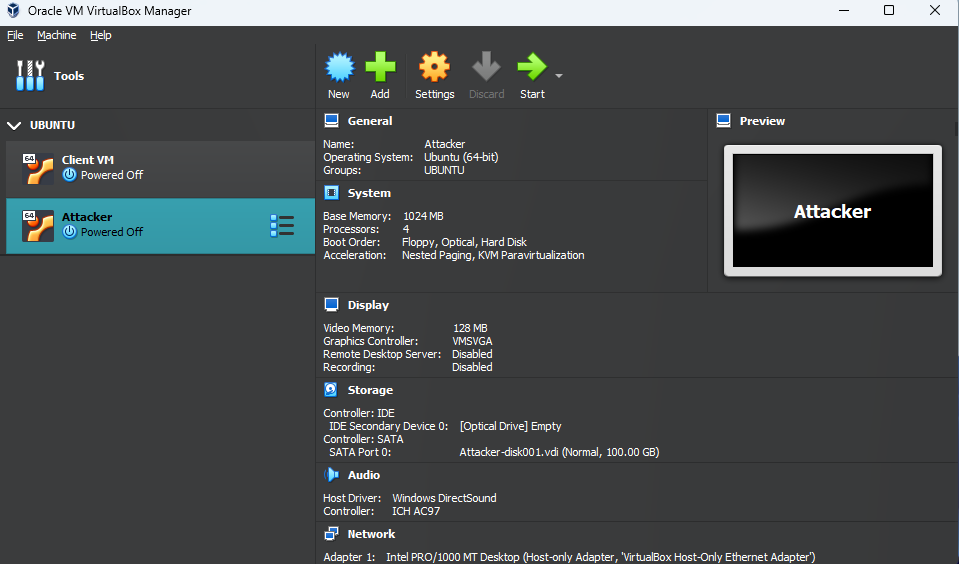
\includegraphics[width=0.9\columnwidth]{graphics/off-path_graphics/virtualbox_manager_client_attacker.png}
    \caption{VirtualBox Manager with Attacker VM freshly imported}
    \label{fig:VirtualBox_Manager_Client_Attacker}
\end{figure}

Select the imported virtual machine instance and click the "Settings" cog in the top-middle of the window. In the window that pops up, under General > Basic > Name, enter "Attacker VM" and then select the "OK" button. The VirtualBox Manager should now look like  Figure~\ref{fig:VirtualBox_Manager_Attacker_Named} below.

\begin{figure}[!h]
    \centering
    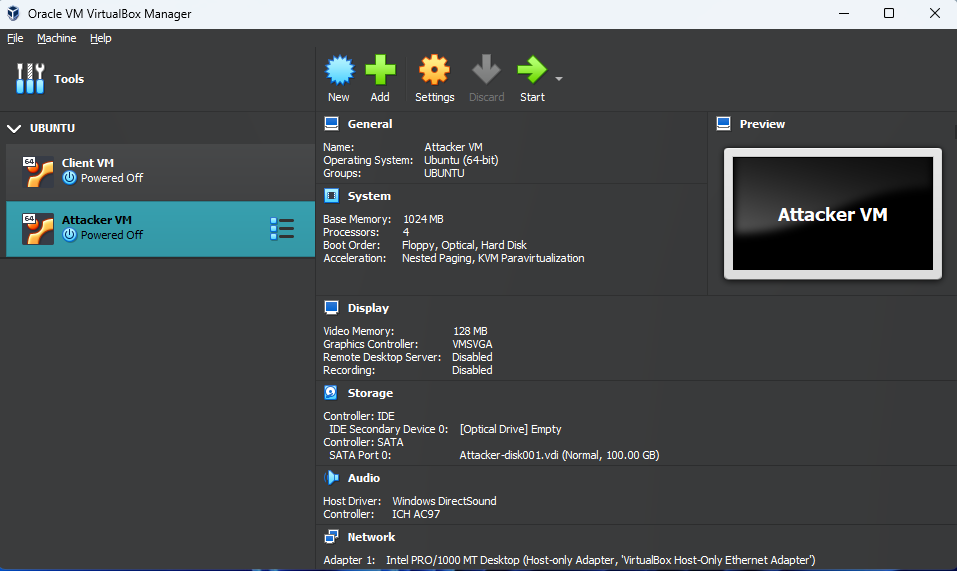
\includegraphics[width=0.9\columnwidth]{graphics/off-path_graphics/virtualbox_manager_attacker_named.png}
    \caption{VirtualBox Manager with Attacker VM properly named}
    \label{fig:VirtualBox_Manager_Attacker_Named}
\end{figure}

\paragraph*{Server Virtual Machine Setup}\label{sec:Virtual-Machine-Server-Virtual-Machine-Setup}
\addcontentsline{toc}{paragraph}{Server Virtual Machine Setup}

From the VirtualBox Manager, click the File option in the menu bar at the top then select the import appliance option from the drop down. Optionally, press Ctrl + i instead to open the Import Virtual Appliance window instead.

Click the yellow folder icon with a green arrow pointing upwards on the middle-right side of the window to open your operating system's file picker. In this file picker, navigate to where you downloaded the virtual machine .ova images to and select "server no update.ova" and then select "Open."

To continue on, click the "Next" and then the "Finish" buttons. This will then start the importing appliance job in VirtualBox. Once the job finishes, you'll see a new virtual machine instance in the left titled "Attacker." The VirtualBox Manager should now look similar to Figure~\ref{fig:VirtualBox_Manager_Client_Attacker_Server} shown below.

\begin{figure}[!h]
    \centering
    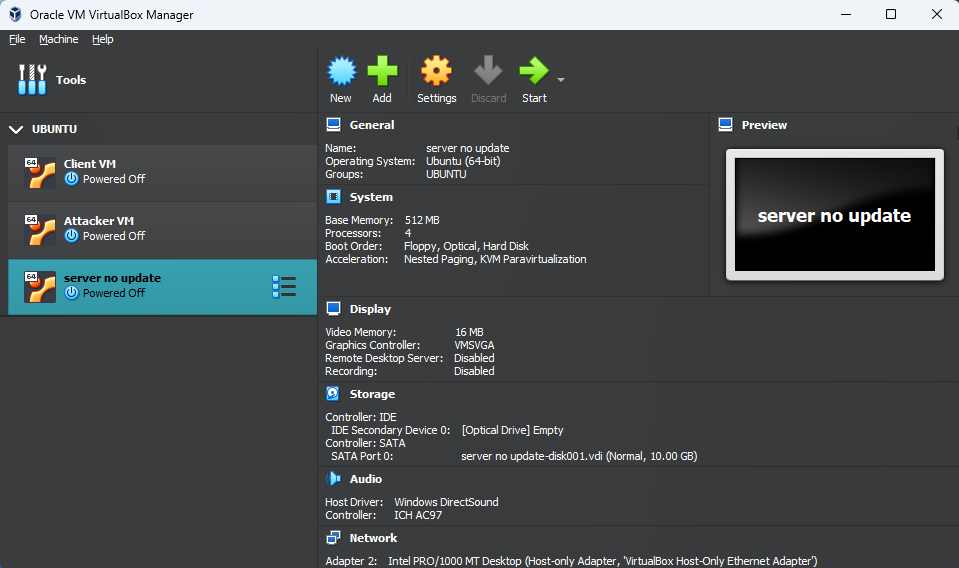
\includegraphics[width=0.9\columnwidth]{graphics/off-path_graphics/virtualbox_manager_server_no_update.png}
    \caption{VirtualBox Manager with Server VM freshly imported}
    \label{fig:VirtualBox_Manager_Client_Attacker_Server}
\end{figure}
Select the imported virtual machine instance and click the "Settings" cog in the top-middle of the window. In the window that pops up, under General > Basic > Name, enter "Server VM" and then select the "OK" button. The VirtualBox Manager should now look like the below Figure~\ref{fig:VirtualBox_Manager_Server_Named} on page ~\pageref{fig:VirtualBox_Manager_Server_Named}.

\begin{figure}[!h]
    \centering
    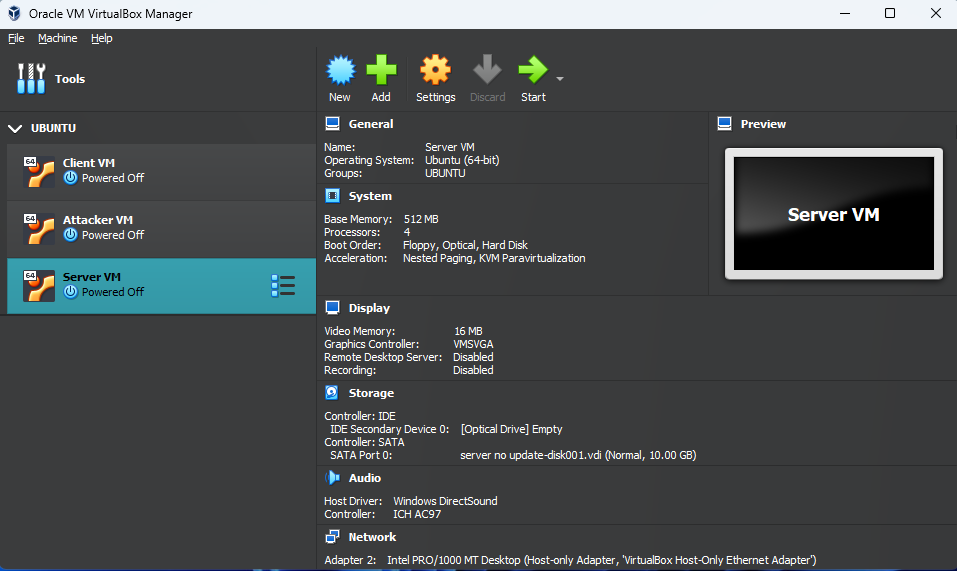
\includegraphics[width=0.9\columnwidth]{graphics/off-path_graphics/virtualbox_manager_server_named.png}
    \caption{VirtualBox Manager with Server VM properly named}
    \label{fig:VirtualBox_Manager_Server_Named}
\end{figure}

\paragraph*{Starting Virtual Machines}\label{sec:Virtual-Machines-Starting-Virtual-Machines}
\addcontentsline{toc}{paragraph}{Starting Virtual Machines}

Now that all three virtual machines for this lab have been created, we need to start them up so we can interact with them throughout the lab.

For each virtual machine instance we've created (Client VM, Attacker VM, and Server VM), select each of them and click the "Start" button that looks like a green arrow pointing to the right, as seen above in Figure~\ref{fig:VM_Start_Button}.

\begin{figure}
    \centering
    
\includegraphics[width=0.3\columnwidth]{graphics/off-path_graphics/vm_start_button.png}
    \caption{The Start button for VM instances}
    \label{fig:VM_Start_Button}
\end{figure}

\textit{Note for Linux users:} Depending on which distribution of Linux you use, VirtualBox may not create a Host-Only Network automatically or may name it differently than the Windows version. To fix this, select "File" > "Tools" > "Network Manager" from the menu bar. This will open up a new section in the VirtualBox Manager. Select the "Host-Only Networks" tab in this new section and click the "Create" button. The defaults should be the same universally but just in case they'll be listed below in Table~\ref{Tab:Host-Only-Network-Info}. Once the Host-only Network is created and configured, go to each VM and change the "Name" field to the name of the Host-only Network that was just created. This field can be found by selecting a VM, and navigating to "Settings" > "Network" and then navigating to whichever adapter (1, 2, 3, or 4) is attached to the "Host-only Adapter."

\begin{table}[!ht]
    \centering
    \begin{tabular}{ |c|@{}c@{}| }
        \hline
         Adapter & DHCP Server \\
         \hline
         \begin{tabular}{c|c}
             Configure Adapter Manually & Selected \\
             \hline
             IPv4 Address & 192.168.56.1 \\
             \hline
             IPv4 Network Mask & 255.255.255.0 \\
             \hline
             IPv6 Address & \textit{Leave blank} \\
             \hline
             IPv6 Prefix Length & 0 \\
         \end{tabular} & \begin{tabular}{c|c}
             Enable Server & Checked \\
             \hline
             Server Address & 192.168.56.100 \\
             \hline
             Server Mask & 255.255.255.0 \\
             \hline
             Lower Address Bound & 192.168.56.101 \\
             \hline
             Upper Address Bound & 192.168.56.254 \\
         \end{tabular} \\
         \hline
    \end{tabular}
    \caption{Host-only Network configuration}
    \label{Tab:Host-Only-Network-Info}
\end{table}

Once the VM's have loaded and the login screen is available, enter "ubuntu" for the password for all three VM's and then hit the "Enter" key to log in. This password will also be the password for any and all sudo commands you enter in the commandline.

\subsubsection*{Connecting Client and Server}
\addcontentsline{toc}{subsubsection}{Connecting Client and Server}

In both the Client VM and Server VM, open a new terminal and make it full screen. In the Client VM, navigate to the path "{\raise.17ex\hbox{$\scriptstyle\mathtt{\sim}$}}/Documents" and in the Server VM, navigate to the path "{\raise.17ex\hbox{$\scriptstyle\mathtt{\sim}$}}/Desktop." In these directories, you'll find "tcp\_server.py" in the Server VM and "tcp\_client.py" in the Client VM.

Note: making the terminals full screen is essential for allowing the python scripts to work correctly. If either one isn't full screen, the scripts will crash.

We'll first need to find the IPv4 addresses of our Server VM. Run the following command in the terminal on the Server VM:
\bigskip
\begin{mdframed}[backgroundcolor=black!10,style=code,nobreak=true,align=center,userdefinedwidth=14cm]
\$ ip a
\end{mdframed}
\bigskip

On the Server VM, the IPv4 address will be under "2: eth0" as the "inet" field. Keep track of this IP address as it will be used later.

Use 6000 as the initial port number. If errors are being received when using port 6000, start incrementing the port by values of 1, 5, or 10 until a valid port is found. Use the following command to start the server on the Server VM:
\bigskip
\begin{mdframed}[backgroundcolor=black!10,style=code,nobreak=true,align=center,userdefinedwidth=14cm]
\$ sudo python3 tcp\_server.py <server\_ip> <server\_port>
\end{mdframed}
\bigskip

If the command was run successfully, the terminal in the Server VM should look similar to Figure~\ref{fig:Server_Waiting_for_Connection} shown below.

\begin{figure}[!h]
    \centering
    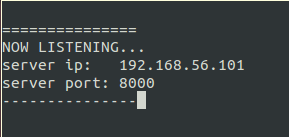
\includegraphics[width=0.6\columnwidth]{graphics/off-path_graphics/server_terminal.png}
    \caption{Server Waiting for Connection}
    \label{fig:Server_Waiting_for_Connection}
\end{figure}

The Client VM can now connect to the server. In the Client VM, using the server ip and server port that shows on the Server VM's terminal, run the following command:
\begin{mdframed}[backgroundcolor=black!10,style=code,nobreak=true,align=center,userdefinedwidth=14cm]
\$ python3 tcp\_client.py <server\_ip> <server\_port>
\end{mdframed}

\bigskip
Your client terminal should look like Figure~\ref{fig:Client_after_connection}, and your server terminal should look like Figure~\ref{fig:Server_after_connection}, both shown on page~\pageref{fig:Client_after_connection}.

\begin{figure}[h]
    \centering
   
    \begin{minipage}{0.49\textwidth}
    \centering
    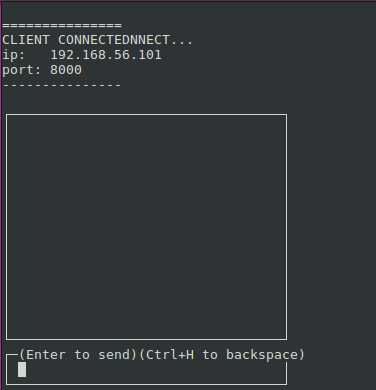
\includegraphics[width=0.81\textwidth]{graphics/off-path_graphics/client_terminal.png}
    \caption{Client Terminal after Connection}
    \label{fig:Client_after_connection}
    \end{minipage}
    \hfill
    \begin{minipage}{0.49\textwidth}
    \centering
    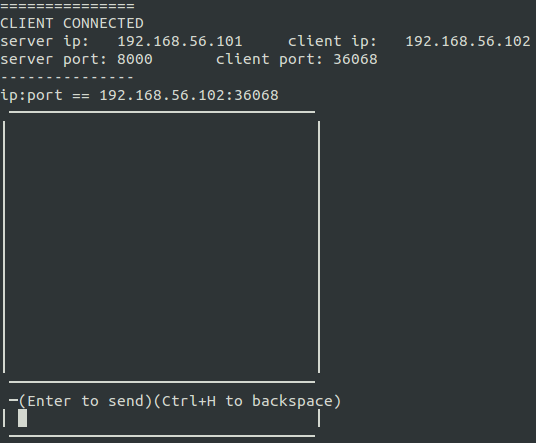
\includegraphics[width=1\textwidth]{graphics/off-path_graphics/server_terminal02_re.png}
    \caption{Server Terminal after Connection}
    \label{fig:Server_after_connection}
    \end{minipage}
\end{figure}

\subsubsection*{Setting Up The Attacker}
\addcontentsline{toc}{subsubsection}{Setting Up The Attacker}

The attacker code is saved in the attacker\_cpp folder in the {\raise.17ex\hbox{$\scriptstyle\mathtt{\sim}$}}/Documents directory. When you alter the code and want to compile it again, remove the file named exploit, then run the make command in the terminal while in the folder.

The attack can then be run from the terminal by typing:

\bigskip
\begin{mdframed}[backgroundcolor=black!10,style=code,nobreak=true,align=center,userdefinedwidth=14cm]
\$ sudo ./exploit <client\_ip> <server\_ip> <server\_port>
\end{mdframed}
\bigskip

The full sequence to remove the old exploit, create a new version, and then execute it can be seen below in two commands.

\bigskip
\begin{mdframed}[backgroundcolor=black!10,style=code,nobreak=true,align=center,userdefinedwidth=14cm]
\$ rm -f exploit \&\& make \\
\$ sudo ./exploit <client\_ip> <server\_ip> <server\_port>
\end{mdframed}
\bigskip

The server port will be the same as the one used to set up the tcp connection. The attack will not work yet though as it is missing code that will be added by you. After attempting the attack on the tcp connection, further attacks on the same connection may be slow or unsuccessful. Restarting the tcp connection of the server and client on a new port will mitigate this. For quick access, all the information needed for the command will be shown on the Server VM's terminal when connected to the Client VM.

\bibliography{References}
\bibliographystyle{plain}

\end{document}

%%%%%%%%%%%%%%%%%%%%%%%%%%%%%%%%%%%%%%%%%